\documentclass[a4paper]{article}

\usepackage[T1]{fontenc}
\usepackage[english]{babel}
\usepackage{graphicx}
\usepackage[nottoc]{tocbibind}
\usepackage[utf8]{inputenc}


%%%reqt stuff
\usepackage{hyperref}
\hypersetup{colorlinks=true, linkcolor=black, urlcolor=blue}
\usepackage[usenames,dvipsnames,svgnames,table]{xcolor}
\definecolor{entityColor}{RGB}{0,100,200}
\definecolor{attributeColor}{RGB}{0,100,50}
\definecolor{relationColor}{RGB}{160,0,30}
\usepackage{listings}
\lstdefinestyle{reqT}{
  belowcaptionskip=1\baselineskip,
  breaklines=true,
  showstringspaces=false,
  basicstyle=\footnotesize\sffamily,
  emph={Ent,Meta,Item,Label,Section,Term,Actor,App,Component,Domain,Module,Product,Release,Resource,Risk,Service,Stakeholder,System,User,Class,Data,Input,Member,Output,Relationship,Design,Screen,MockUp,Function,Interface,State,Event,Epic,Feature,Goal,Idea,Issue,Req,Ticket,WorkPackage,Breakpoint,Barrier,Quality,Target,Scenario,Task,Test,Story,UseCase,VariationPoint,Variant},
  emphstyle=\bfseries\color{entityColor},
  emph={[2]has,is,superOf,binds,deprecates,excludes,helps,hurts,impacts,implements,interactsWith,precedes,requires,relatesTo,verifies},
  emphstyle={[2]\bfseries\color{relationColor}},
  emph={[3]Attr,Code,Constraints,Comment,Deprecated,Example,Expectation,FileName,Gist,Image,Spec,Text,Title,Why,Benefit,Capacity,Cost,Damage,Frequency,Min,Max,Order,Prio,Probability,Profit,Value,Status},
  emphstyle={[3]\color{attributeColor}},  
}
\lstset{style=reqT}




%%%end reqt stuff




\title{System Requirements}
\author{Group D}
\date{\today}

\begin{document}
	\maketitle
	\thispagestyle{empty}
	\setcounter{page}{0}
	\pagebreak
	\tableofcontents
	\pagebreak
	



	\section{Background} % (fold)
	\label{sec:background}
	
		\subsection{Costumer relationship}
			We have a close relationship to our costumers, with frequent meetings at least once a week. Outside these, most of the communication is done by mail. The meetings are done with open discussions and not to formal. 

			The costumer is the product owner for the system.


	% section background (end)

	\section{System Purpose} % (fold)
	The purpose of the system is to make everyday travels an easier task for people using public transportation. The users of this application will have an easily accessible overview of how long it will take them to get to their favourite locations. These locations can be their work, home, the gym etc.
	
	
The project goal is to develop an app and/or widget where the user can see how to get to their favorite destinations in the shortest time possible. The shown travel alternatives shall be adjusted according to the current position of the user, by the starting point being set to the users graphical location.
	\section{Domain}
		\begin{figure}[h]
				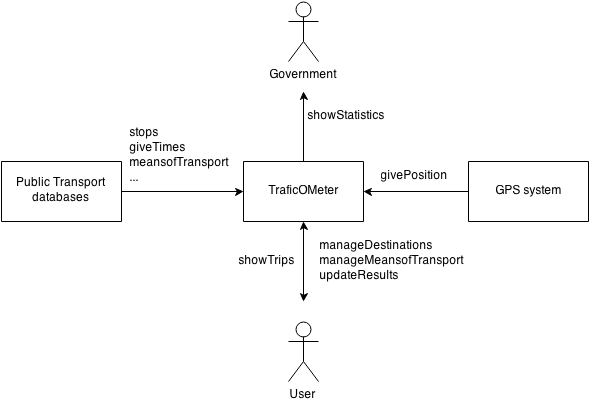
\includegraphics[scale=0.65]{Context-v1.png}
			\caption{Context Diagram for the system}
		\end{figure}
		\subsection{Parts of the context diagram} % (fold)
		\label{sub:parts_of_the_context_diagram}
		\begin{itemize}
			\item[Government agency] The part of the government that is interested in public transport. 
			\item[User] Anyone using the app.
			\item[GPS system] The native GPS of the device or WI-FI location services.
			\item[RPTD] Regional public transport databases, provides information regarding time tables and delays.
			\item[TrafficOmeter] This is the product.
		\end{itemize}
		\subsection{Transitions} % (fold)
		\label{sub:transitions}
			\subsubsection{Traffic information} % (fold)
			\label{ssub:traffic_information}
			This section covers the different traffic information that is sent from the regional public transport databases to the TrafficOmeter system.
			\begin{itemize}
				\item[Stops] The geographical positions where it is possible to get on and off public transport.
				\item[GiveTimes] The time table for the routes included in the updated trips.
				\item[MeansOfTransport] The means of transportations that are represented in the updates trips.
			\end{itemize}
			% subsubsection traffic_information (end)
		% subsection transitions (end)
		% subsection parts_of_the_context_diagram (end)
		
	
	
	\section{Requirements}
		\subsection{Goal Level Requirements}
			

\begin{lstlisting}
Stakeholder SwedishGovernment
	Goal MoreTravel
		Spec Increase the use of public transportation by making it a more effortless to find travel connections
	Goal UserTravelStatistics
		Spec The government wants statistics relevant for research purposes, to improve future infrastructure
	Goal AccessibleForEverybody
		Spec As the government is supporting the project it needs to be developed for all Swedish citizens and tourists in Sweden
Stakeholder User
	Goal TravelOverview
		Spec The user wants to have an overview over the fastest possible route to their frequently visited destinations
	Goal MinimalUserMaintenance
		Spec The user wants to know the total time to get to a frequently visited destinations without having to manually insert information every time
	Goal UserTiedInformation
		Spec The information should be connected to the user and not tied to the user's device
Stakeholder ProductOwner
	Goal ReturnOnInvestment
		Spec The product needs to create enough value for the users, so that the product owner can benefit from their investment
	Goal ReplaceCurrentSoftware
		Spec The product owner wants the system to support the functions that appeal to the users, in such way that they will use the product as their main search tool for transports.
Stakeholder RegionalPublicTransportationAdministrators
	Goal UserTravelStatistics
		Spec The system will provide data about the users' possible travels that can be analyzed to reveal flaws in the local transportation systems

\end{lstlisting}
		\subsection{Domain Level Requirements}
			\subsubsection{Tasks}
				

\begin{lstlisting}
Task addDestination
  Spec User saves a geographical location
Trigger: User want another destination to travel to
  Task Find Geographical Location
    Spec Locate a geographical location to travel to
    Variant Select current GPS-coordinates as geographical location
    Variant Desired geographical location does not exist
    Variant Multiple matches for geographical location query
    Frequency 5
  Task Name Geographical Location
    Spec Give a name to a geographical location
    Frequency 1
  Task Save Geographical Location
    Spec Save a geographical location to the device and database
    Frequency 1
  Why The user shall not have to search for a geographical location he/she might visit multiple times.
  Frequency 3
Task chooseTransportationMeans
  Spec User specifies which means of transportation(s) that the system shall use for calculating the fastest trip
  Frequency 1
Task removeDestination
  Spec Remove a previously added destination
  Task SelectDestination
    Spec Select a destination from a list of destinations
    Frequency 1
  Task deleteSelectedDestination
    Spec Remove a selected destination
    Frequency 1
  Frequency 1

\end{lstlisting}
			\subsubsection{Feature Requirements}
				\begin{lstlisting}

\end{lstlisting}


			 \paragraph{Statistics}


\begin{lstlisting}
Feature GetPopularMeansOfTransportStatistics
	Spec The system shall be able to extract the most preferable means of transportation for different routes
	Why The information could be used for future planning of the infrstructure. eg. If there are both trains and buses between Point A and Point B and almost everyone uses the train, then the buses might be excessive
	Example The statistiscs could be extracted using a web interface, on the format specified in Data Requirement ExtractingFormat
	Cost 128
	Stakeholder Costumer
		Benefit 2
	Stakeholder User
		Benefit 0
	Stakeholder Government
		Benefit 25
Feature GetPopularLocationStatistics
	Spec The system shall be able to provide statistics about which geographical locations are popular
	Why The Swedish government hopes to be able to use this and other statistics as decision basis when planning infrastructure
	Cost 128
	Example The system supervisor(s) provides the Swedish government with the extracted statistics
	Stakeholder Customer
		Benefit 2
	Stakeholder User
		Benefit 0
	Stakeholder Government
		Benefit 15
Feature GetUserStatistics
	Spec The system shall be able to extract user statistics of the System
	Why The information could be used to get an overview of what might be changed about the app or if the app is used at all
	Example The statistiscs could be extracted using a web interface, on the format specified in Data Requirement ExtractingFormat
	Cost 128
	Stakeholder Costumer
		Benefit 2
	Stakeholder User
		Benefit 0
	Stakeholder Government
		Benefit 2
Feature GetTravelStatistics
	Spec The system shall be able to extract information about frequent travels between point A and point B
	Why The information could be used for future planning of the infrastructure. If travels between point A and B occurs frequently, then it might say something about the load of this route
	Example The statistiscs could be extracted using a web interface, on the format specified in Data Requirement ExtractingFormat
	Cost 128
	Stakeholder Costumer
		Benefit 2
	Stakeholder User
		Benefit 0
	Stakeholder Government
		Benefit 25
Feature GetRoutesStatistics
	Spec The system shall be able to provide statistics about which routes that all users has at a specific time
	Why This information could be used to extract information about the infrastructure in a specific city. From the information things like number of transfers, the given time it takes relative to the distance covered etc. could be useful
	Cost 128
	Example The system supervisor(s) checks the current traffic information in a given city
	Stakeholder Costumer
		Benefit 2
	Stakeholder User
		Benefit 0
	Stakeholder Government
		Benefit 0

\end{lstlisting}
		
				
			 \paragraph{ServerToClientCommunication}


\begin{lstlisting}
Feature MultiAccessibleUserData
	Spec A single user shall be able to access its information from multiple devices
	Why User might want to use multiple smartphones and/or tablets, or have obtained a new smartphone or tablet
	Example The system could support a user profile and a server storage solution so that the user can get its information using multiple devices
	Stakeholder User
		Benefit 7
	Cost 64
	Stakeholder SwedishGovernment
		Benefit 3
Feature KeepAcountPrivate
	Spec A user can only access its own destinations
	Why The data is private and shall not be possible view or change by someone else
	Cost 32
	Example The system could provide a login system that protects the data

\end{lstlisting}
		
				
			 \paragraph{Maintenance}


\begin{lstlisting}
Feature SaveDestination
	Spec The user can save a destination to its list of already saved destinations for easy access
	Why To populate the list of destinations
	Example Add button in the application
	Cost 32
	Stakeholder Customer
		Benefit 5
	Stakeholder User
		Benefit 15
	Stakeholder SwedishGovernment
		Benefit 8
Feature SpecifyLocationByMap
	Spec The user can specify the location by moving a target pin on a map
	Why A map gives more information to the user and makes is easier for the user to communicate its wishes
	Example Use third party map software
	Cost 64
	Stakeholder Customer
		Benefit 2
	Stakeholder User
		Benefit 3
	Stakeholder SwedishGovernment
		Benefit 1
Feature SpecifyMeansOfTravel
	Spec The user shall be able to specify which of the supported means of transportation it would like to use and then the system shall use the selected means of transportation
	Why Not all users want to use the same means of travel
	Example This can be implemented using a settings dialog
	Cost 4
	Stakeholder Customer
		Benefit 4
	Stakeholder User
		Benefit 9
	Stakeholder SwedishGovernment
		Benefit 4
Feature SpecifyLocationByAddress
	Spec The user shall be able to specify a location by providing an address
	Why The user might need to travel to a specific address
	Example A text input field, incorporate the Google maps search engine
	Cost 64
	Stakeholder Customer
		Benefit 5
Feature ChangeNameOnDestination
	Spec It shall be possible to change the name of a destination
	Why To make it easier to tell the different destinations apart a user might want to change the name of a destination. For example, a user want to change the name of the destination that correlates to the users work to the name: WORK
	Example An EDIT button besides the field for the name of the destination
	Cost 8
	Stakeholder User
		Benefit 1
	Stakeholder SwedishGovernment
		Benefit 0
Feature DeleteDestination
	Spec It shall be possible for the user to remove a previously saved destination
	Why If that destination no longer is in the interest of the user it shall be possible to remove it
	Example An Delete button besides the name of the destination
	Cost 8
	Stakeholder Customer
		Benefit 4
	Stakeholder User
		Benefit 2
	Stakeholder SwedishGovernment
		Benefit 0
Feature MultipleDestinations
	Spec The user shall be able to store multiple destinations
	Why It is very useful that the user can store several destinations at the same time without having to do a new search every time the user wants to go somewhere
	Example Multiple fields of destinations
	Cost 8
	Stakeholder Customer
		Benefit 4
	Stakeholder User
		Benefit 7
	Stakeholder SwedishGovernment
		Benefit 3
Feature OrderDestinations
	Spec It shall be possible for the user to order its destinations in an priority order
	Why The screen of a smart phone might not be big enough to display all	of a users destinations. Therefore it would be convenient for the user to order its destination in an priority order
	Example A ORDER alternative in the settings for the widget where the user is able to drag and drop its destinations up and down to match the actual view on the widget
	Cost 16
	Stakeholder Customer
		Benefit 5

\end{lstlisting}
		
				
			 \paragraph{Support}


\begin{lstlisting}
Feature Language
	Spec The system shall have support for both Swedish and English
	Why To make the product available for more people
	Example A setting where one can use the language to be used
	Cost 64
Feature Android
	Spec The system shall support Android
	Why A big share of the smart phone and tablet market uses the Android operating system
	Cost 64
	Stakeholder User
		Benefit 5
Feature IOS
	Spec The system shall support IOS
	Why A big share of the smart phone and tablet market uses the IOS operating system
	Cost 64
	Stakeholder User
		Benefit 5

\end{lstlisting}
		
				
			 \paragraph{Usage}


\begin{lstlisting}
Feature ViewNextOption
	Spec The user shall be able to choose to discard the displayed trip to a destination and instead get the next trip to the same destination
	Why Because the time to the fastest alternative may not be enough for the user to get ready to leave
	Example Get the second fastest option by swiping the current option for the destination off the screen
	Cost 8
	Stakeholder Customer
		Benefit 4
Feature FastestTrip
	Spec The system shall automatically show the total travel time of the fastest trip
	Why So the user can see how long time it takes to travel to the destinations
	Example Show a list of destinations and in this list show the time it takes to get to the different alternatives
	Cost 2
	Stakeholder Customer
		Benefit 5
	Stakeholder User
		Benefit 9
	Stakeholder SwedishGovernment
		Benefit 10
Feature GeographicalStartingPoint
	Spec The system shall be able to use the user's geographical location as a starting point for a trip
	Why The position shall be used as the starting point when determining the route
	Example Use native GPS or WiFi-positioning feature of platforms
	Cost 32
	Stakeholder Customer
		Benefit 3
Feature ShowRouteToFirstStop
	Spec When the user selects a specific travel option the route between the current position and the first stop shall be accessible
	Why The user might not find its way in the current area, and shall be able to get to the first stop quickly
	Example Show the route between current position and first stop on a map.
	Cost 16
	Stakeholder Customer
		Benefit 3
	Stakeholder User
		Benefit 8
	Stakeholder SwedishGovernment
		Benefit 4
Feature MaxDistToStop
	Spec The user shall be able to specify the maximum distance in a transfer between two adjacent stops.
	Why The user might not want to walk several minutes between stops in a transfer
	Cost 32
	Stakeholder Customer
		Benefit 4
Feature MinWaitTime
	Spec The user shall be able to specify the minimum waiting time in a transfer between two adjacent stops.
	Why The user might want to be guaranteed some time for the transfers to not feel stressed
	Cost 32
	Stakeholder Customer
		Benefit 4

\end{lstlisting}
		
				
			 \paragraph{MeansOfTransportation}


\begin{lstlisting}
Feature SupportBuses
	Spec The System shall retrieve information for all bus lines in Sweden that has an accessible API
	Why To support as many bus lines as possible
	Cost 128
	Stakeholder Customer
		Benefit 5
Feature SupportTrains
	Spec The System shall retrieve information for all train lines in Sweden that has an accessible API
	Why To support as many train lines as possible
	Cost 128
	Stakeholder Customer
		Benefit 5
Feature SupportFerries
	Spec The System shall retrieve information for all ferry lines in Sweden that has an accessible API
	Why To support as many ferry lines as possible
	Cost 128
	Stakeholder Customer
		Benefit 5

\end{lstlisting}
		
				
			 \paragraph{Interfaces}


\begin{lstlisting}
Feature ExtractDataFromProviders
	Spec Extract travel data from regional public transportation administrators
	Why Obtaining travel data from this source is a vital part of our system, since it is used in all calculations
	Cost 256
	Example If the user wants to know the fastest trip to its home, the system will need the time tables of all the transportation means involved

\end{lstlisting}				
			
		\subsection{Product Level Requirements}		
			\subsubsection{Data Requirements}
				The data in the data model should be stored by the system.	
				\begin{figure}[h]
					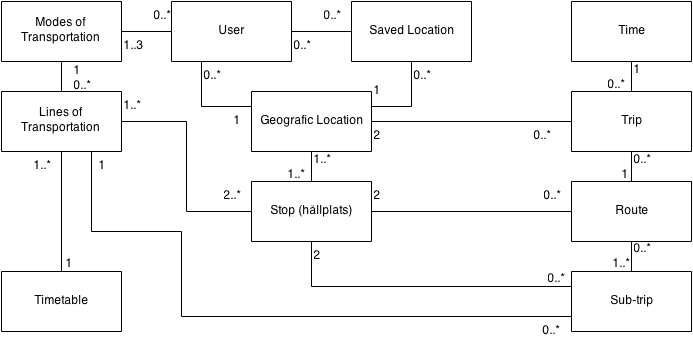
\includegraphics[scale=0.50]{datamodel-v1.png}
					\caption{Data Model for the system}
				\end{figure}
				
				
				
\begin{lstlisting}
Product Our Product
  Term Route
    Spec The path between two different stops. Consists of one or more 'sub-trip's
  Term Trip
    Spec A specific travel between two geographical (GPS) points
    Example Between a users current position and one of its saved destinations
  Term Line
    Spec A set of 'stop's that is served by the same vehicle
    Example Bus 6 between X and Y
  Term Sub-trip
    Spec A subset of a line that is part of a bigger 'trip'
    Example Bus 3, stop #4 to stop #9

\end{lstlisting}
			\subsubsection{Functional Requirements}
				

\begin{lstlisting}
Feature GeographicLocation
  Spec The system should be able to get the current geographical position of the user
  Why The position is used to be able to calculate the whole trip since the system is supposed to say 'to home in 20 minutes' 
  Example Use native GPS or WiFi-positioning feature of platforms
  Status ELICITED
  Stakeholder Customer
    Benefit 5

\end{lstlisting}
		
				\textbf{låg under feature innan, men har nog aldrig sorteras så dessa ska in under rätt rubriker sen}
			
				\begin{itemize}
					\item Req("MeansOfTransportation") has (Spec("The User shall be able to specify which of the supported means of transportation it would like to use and then the system shall use the selected means of transportation")), \textbf{Kanske borde göras om till ett subkrav, om någon vet hur man gör detta}. 
					\item Req(''MaxDistBetweenStops'') has (Spec(''The user shall be able to specify the max distance between stops that the system shall take in to acount when calculating the route. If no route can be found, the system can ignore the contraint'')), \textbf{var ska denna vara, kan behövas finslipas}


					\item The User shall be able to select another travel option if the shown alternative does not fit its needs. This 				is preferably done by swiping through different available alternatives. \textbf{Det fanns in feature, och är nu ändrat där för att passa bättre, den heter ViewNextOption, kolla och kommentera om nödvändigt."})),
					\item Req("TimeToDestinationsOnMainScreen") has (Spec("The User shall be able to see the time to reach it's saved destinations on the main screen of the device.")), \textbf{har ett liknande i features, men borde formulera till nåt mellanting}
				\end{itemize}	
					
					
				\textbf{Det här hör förmodligen inte hemma här men måste finnas med någonstans på något sätt.}
				\begin{itemize}
					\item The User shall be able to choose means of transportation from ferry, bus and train. They must choose at least one. \textbf{lägga till krav på minst en någonstans och ta bort resten?, finns i princip i tasks men måste skrivas om till något tydligt}
					\item A destination consists of a name (lägga till i data modellen), gps-position \textbf{finns detta i datamodel nu??}
				\end{itemize}
	\subsection{Design Level Requirements}
	\section{Quality Requirements}
		When it comes to quality we consider the issues prioritized in the following way:
		
		\begin{tabular}{|l|c|c|c|c|c|}
			\hline
			& Critical & Important & As usual & Unimportant & Ignore \\
			\hline			
			\multicolumn{6}{|l|}{\textbf{Operation}} \\	
			\hline
			Integrity/Security & & 1 & & & \\
			\hline
			Correctness & & & x & & \\			
			\hline
			Reliability/Availability & & 2 & & & \\
			\hline
			Usability & 3 & & & & \\
			\hline
			Efficiency & & 4 & & & \\
			\hline
			\multicolumn{6}{|l|}{\textbf{Revision}} \\
			\hline
			Maintainability & & & x & & \\
			\hline
			Testability & & & x & & \\
			\hline
			Flexibility & & & & 5 & \\
			\hline
			\multicolumn{6}{|l|}{\textbf{Transition}} \\
			\hline
			Portability & 6 & & & & \\
			\hline
			Interoperability & & 7 & & & \\
			\hline
			Reusability & & & x & & \\
			\hline
		\end{tabular}

		\subsection{Goal Level Requirements}
		\subsection{Domain Level Requirements}
		\begin{itemize}
			\item 	Req("Android") has (Spec("The system shall support Android")),
			\item	Req("IOS") has (Spec("The system shall support IOS")),
		\end{itemize}
		\subsection{Product Level Requirements}
			\begin{lstlisting}

\end{lstlisting}


       \section{Usability}


\begin{lstlisting}
Quality UpdateStartView
  Spec Updating start view shall be possible with one press of a button per time
  Stakeholder Customer
    Prio 2

\end{lstlisting}
    
        
       \section{Efficiency}


\begin{lstlisting}
Quality GPS-position
  Spec The system shall give a GPS-position correct within a 50 meter radius
  Stakeholder Customer
    Prio 4
Quality TransferTime
  Spec The product will not have transfers of less than 5 minutes
  Stakeholder Customer
    Prio 3
Quality requestCapacity
  Spec The system needs to be able to process at least 20000 update requests per minute

\end{lstlisting}
    
        
       \section{Reliability}


\begin{lstlisting}
Quality Uptime-Reliability
  Spec The system should have an uptime of 99%

\end{lstlisting}
    
        
       \section{Security}


\begin{lstlisting}
Quality UserIntegrity
  Spec The system should not provide any statistics that could be used to track a single users travel habits or specific user positions
  Stakeholder Customer
    Prio 5

\end{lstlisting}		
		\subsection{Design Level Requirements}	
	\section{Prioritization}
		\subsection{100 dollar method -  importance}
		\textbf{prio för resten av stakeholder behövs också, be kund om prio imorn om vi hinner}
		\textbf{måste lägga in resten av kraven också och då göra om importace gissningarna}
		\begin{tabular}{|l|c|c|}
			\hline
			&User	&Staten \\
			\hline			
			Visability	&13	&7 \\
			\hline
			reach from devices	&2	&2 \\
			\hline
			Geografic location	&9	&4 \\
			\hline
			show total travel time	&9	&10 \\
			\hline
			save location	&15	&7 \\
			\hline
			select by map	&3	&1 \\
			\hline
			means of travel	&9	&4 \\
			\hline
			portability	&10	&14 \\
			\hline
			remove destination	&2	&0 \\
			\hline
			multiple saved dest	&7	&3 \\
			\hline
			change name	&1	&0 \\
			\hline
			show route to first stop	&8	&4 \\
			\hline
			statistics	&0	&25 \\
			\hline
			uptime	&5	&14 \\
			\hline
			gps accuracy	&7	&5 \\
			\hline			
			
		\end{tabular}

	\subsection{Cost}
		Gjort för developers		
		\begin{tabular}{|l|c|c|}
			\hline
		
			&cost insertion sort- minst kostnad &cost100 \\
			\hline
			Visability	&9	&7 \\
			\hline
			reach from devices	&12	&11 \\
			\hline			
			Geografic location	&6	&4 \\
			\hline
			show total travel time	&5	&3 \\
			\hline
			save location	&3	&1 \\
			\hline
			select by map	&7	&4 \\
			\hline
			means of travel	&10	&8 \\
			\hline
			portability	&14	&13 \\
			\hline
			remove destination	&1	&1 \\
			\hline
			multiple saved dest	&4	&2 \\
			\hline
			change name	&2	&1 \\
			\hline
			show route to first stop	&11	&10 \\
			\hline
			statistics	&13	&12 \\
			\hline
			uptime	&15	&18 \\
			\hline
			gps accuracy	&8	&5 \\
			\hline
		\end{tabular}
\end{document}
